\documentclass[11pt,letterpaper]{article}
\usepackage[margin=1in]{geometry}
\usepackage{amsmath,amssymb}
\usepackage{booktabs}
\usepackage{longtable}
\usepackage{graphicx}
\usepackage{hyperref}
\usepackage{xcolor}
\usepackage{listings}
\usepackage{tikz}
\usetikzlibrary{shapes,arrows,positioning,fit,backgrounds}
\usepackage{fancyhdr}
\usepackage{titlesec}

\hypersetup{
    colorlinks=true,
    linkcolor=blue!60!black,
    urlcolor=blue!60!black
}

\pagestyle{fancy}
\fancyhf{}
\rhead{Yale Budget Lab}
\lhead{Tariff Model Dependency Map}
\rfoot{Page \thepage}

\titleformat{\section}{\Large\bfseries\color{blue!60!black}}{\thesection}{1em}{}
\titleformat{\subsection}{\large\bfseries}{\thesubsection}{1em}{}

\lstset{
    basicstyle=\ttfamily\small,
    backgroundcolor=\color{gray!10},
    frame=single,
    framerule=0pt,
    breaklines=true
}

\title{\textbf{Yale Budget Lab Tariff Model}\\[0.5em]\Large Dependency Map and Calculation Reference}
\author{Generated from \texttt{ricco\_tariffs\_11-17.xlsm}}
\date{January 5, 2026}

\begin{document}

\maketitle
\tableofcontents
\newpage

%==============================================================================
\section{Overview}
%==============================================================================

This document maps the calculation dependencies in the Budget Lab's tariff model Excel workbook. Each result is traced back to its inputs and intermediate calculations to facilitate conversion to R.

\subsection{Model Structure}

The workbook contains 34 worksheets organized into three layers:
\begin{itemize}
    \item \textbf{Input Layer:} Tariff parameters, import data, external model outputs
    \item \textbf{Calculation Layer:} ETR computation, price effects, revenue scoring
    \item \textbf{Output Layer:} Key Results, tables (T1, T3), figures (F1--F7)
\end{itemize}

%==============================================================================
\section{Effective Tariff Rates}
%==============================================================================

\subsection{Pre-Substitution ETR (Increase)}

\begin{tabular}{ll}
\toprule
\textbf{Output Cell} & \texttt{Key Results!B3} \\
\textbf{Value} & 14.4\% \\
\bottomrule
\end{tabular}

\vspace{1em}
\noindent\textbf{Dependency Chain:}
\begin{lstlisting}
Key Results!B3
  -> 'F1 Historical'!F239
       -> = F236 - E236
            F236 = E237 (All-In Pre-Sub ETR)
            E236 = B236 (Baseline ETR = 2.418%)
\end{lstlisting}

\noindent\textbf{Calculation:}
\begin{equation}
\text{ETR}_{\text{increase}} = \text{ETR}_{\text{all-in}} - \text{ETR}_{\text{baseline}}
\end{equation}

\subsection{Pre-Substitution ETR (All-In)}

\begin{tabular}{ll}
\toprule
\textbf{Output Cell} & \texttt{Key Results!B4} \\
\textbf{Value} & 16.8\% \\
\bottomrule
\end{tabular}

\vspace{1em}
\noindent\textbf{Dependency Chain:}
\begin{lstlisting}
Key Results!B4
  -> 'F1 Historical'!F237
       -> = E237
            -> = B236 + ricco_price_effects_and_etr!D25 * 100
                 B236 = 2.418 (Baseline ETR)
                 D25 = BW55/100 (Weighted ETR)
\end{lstlisting}

\noindent The weighted ETR is computed as:
\begin{equation}
\text{ETR}_{\text{weighted}} = \frac{\sum_{c} \text{ETR}_c \times \text{Import}_c}{\sum_{c} \text{Import}_c}
\end{equation}

where $c \in \{\text{China, Canada, Mexico, UK, Japan, EU, ROW, FTROW}\}$.

\subsection{Post-Substitution ETR}

\begin{tabular}{lll}
\toprule
\textbf{Metric} & \textbf{Cell} & \textbf{Value} \\
\midrule
Increase & \texttt{Key Results!B7} & 11.9\% \\
All-In & \texttt{Key Results!B8} & 14.4\% \\
\bottomrule
\end{tabular}

\vspace{1em}
\noindent Post-substitution values use row 25 of \texttt{ricco\_price\_effects\_and\_etr} instead of row 24, reflecting import substitution responses.

\subsection{ETR Input Sources}

\begin{longtable}{p{3cm}p{5cm}p{6cm}}
\toprule
\textbf{Input} & \textbf{Location} & \textbf{Description} \\
\midrule
\endhead
Baseline ETR & \texttt{F1 Historical!B236} & 2.418\% (2024 baseline) \\
Country ETRs & \texttt{Weighted US Tariff!Z83:AG127} & Matrix: GTAP sector $\times$ country \\
Import weights & \texttt{ricco\_price\_effects!BE:BL} & Country import shares from GTAP \\
Country mapping & \texttt{Weighted US Tariff!Z82:AG82} & china, canada, mexico, uk, japan, eu, row, ftrow \\
\bottomrule
\end{longtable}

%==============================================================================
\section{Price Effects}
%==============================================================================

\subsection{Consumer Price Increase (Pre-Substitution)}

\begin{tabular}{ll}
\toprule
\textbf{Output Cell} & \texttt{Key Results!B12} \\
\textbf{Value} & 1.2\% \\
\bottomrule
\end{tabular}

\vspace{1em}
\noindent\textbf{Dependency Chain:}
\begin{lstlisting}
Key Results!B12
  -> ricco_price_effects_and_etr!E24
       -> = (D24 * -B13 * F24 * H24)
          + (D24*100) * H24 * F24 * (1+B14) / 100
\end{lstlisting}

\noindent\textbf{Formula:}
\begin{equation}
\Delta P = \underbrace{\tau \cdot (-\delta) \cdot \alpha_g \cdot \alpha_m}_{\text{USD offset effect}} + \underbrace{\tau \cdot \alpha_m \cdot \alpha_g \cdot (1 + \phi)}_{\text{Passthrough effect}}
\end{equation}

where:
\begin{itemize}
    \item $\tau$ = Effective tariff rate
    \item $\delta$ = USD offset (0.17)
    \item $\phi$ = Domestic price passthrough (0.50)
    \item $\alpha_g$ = Goods share of PCE (0.31)
    \item $\alpha_m$ = Import share of goods PCE (0.21)
\end{itemize}

\subsection{Per-Household Cost}

\begin{tabular}{lll}
\toprule
\textbf{Metric} & \textbf{Cell} & \textbf{Value} \\
\midrule
Pre-Substitution & \texttt{Key Results!B13} & \$1,671 \\
Post-Substitution & \texttt{Key Results!B15} & \$1,257 \\
\bottomrule
\end{tabular}

\vspace{1em}
\noindent\textbf{Dependency Chain:}
\begin{lstlisting}
Key Results!B13
  -> -ricco_price_effects_and_etr!I24
       -> I24 = 'F6 Distribution (C)'!N23
            -> N23 = AVERAGE(B23:K23)
                     [Average cost across income deciles]
\end{lstlisting}

\subsection{Price Effect Parameters}

\begin{longtable}{llcp{6cm}}
\toprule
\textbf{Parameter} & \textbf{Cell} & \textbf{Value} & \textbf{Description} \\
\midrule
\endhead
USD Offset & \texttt{B13} & 0.17 & $= 0.3 \times 0.58$ (exchange rate adjustment) \\
Price Passthrough & \texttt{B14} & 0.50 & Domestic price passthrough rate \\
Goods Share of PCE & \texttt{B15} & 0.31 & Share of consumption on goods \\
Import Share & \texttt{B16} & 0.21 & Import share of goods consumption \\
\bottomrule
\end{longtable}

%==============================================================================
\section{Revenue Estimates}
%==============================================================================

\subsection{Conventional Revenue (10-Year)}

\begin{tabular}{ll}
\toprule
\textbf{Output Cell} & \texttt{Key Results!B18} \\
\textbf{Value} & \$2,728 billion \\
\bottomrule
\end{tabular}

\vspace{1em}
\noindent\textbf{Dependency Chain:}
\begin{lstlisting}
Key Results!B18
  -> 'T3 Fiscal'!L6
       -> = SUM(B6:K6)  [FY2026-FY2035]
            -> B6 = 'Fiscal Summary'!C28
                 -> C28 = C25 + C27 + C26
                      C25 = Gross revenue
                      C26 = Compliance effect (-10%)
                      C27 = Income effect (-23%)
\end{lstlisting}

\noindent\textbf{Revenue Formula:}
\begin{equation}
R_{\text{net}} = \underbrace{(D_{\text{new}} - D_{\text{baseline}})}_{\text{Gross Revenue}} \times \underbrace{(1 - 0.10 - 0.23)}_{\text{Behavioral adjustments}}
\end{equation}

where:
\begin{align}
D_{\text{new}} &= \text{ETR}_{\text{new}} \times M_{\text{adjusted}} \\
M_{\text{adjusted}} &= M_{\text{baseline}} \times (1 - \varepsilon \cdot \Delta\tau)
\end{align}

\subsection{Dynamic Revenue (10-Year)}

\begin{tabular}{ll}
\toprule
\textbf{Output Cell} & \texttt{Key Results!B19} \\
\textbf{Value} & \$2,342 billion \\
\bottomrule
\end{tabular}

\vspace{1em}
\noindent\textbf{Calculation:}
\begin{equation}
R_{\text{dynamic}} = R_{\text{conventional}} + \sum_{t=2026}^{2035} \Delta_t^{\text{dynamic}}
\end{equation}

The dynamic scoring adjustments $\Delta_t^{\text{dynamic}}$ are stored in \texttt{T3 Fiscal!B8:K8}.

\subsection{Revenue Input Sources}

\begin{longtable}{p{3.5cm}p{4cm}p{6cm}}
\toprule
\textbf{Input} & \textbf{Source} & \textbf{Description} \\
\midrule
\endhead
Baseline Imports & \texttt{Fiscal Summary!C16} & CBO January baseline (\$4,283B for FY2026) \\
Baseline Duties & \texttt{Fiscal Summary!C17} & CBO baseline duties (\$84B) \\
Import Elasticity & \texttt{Fiscal Summary!C42} & Response of imports to tariffs \\
Compliance Effect & Hard-coded & $-10\%$ of gross revenue \\
Income Effect & Hard-coded & $-23\%$ of gross revenue \\
Dynamic Effects & \texttt{T3 Fiscal!B8:K8} & Year-by-year dynamic adjustments \\
\bottomrule
\end{longtable}

%==============================================================================
\section{Macroeconomic Effects}
%==============================================================================

\subsection{GDP Impact}

\begin{tabular}{llll}
\toprule
\textbf{Metric} & \textbf{Cell} & \textbf{Value} & \textbf{Period} \\
\midrule
Q4-Q4 GDP & \texttt{Key Results!B22} & $-0.50\%$ & 2025 \\
Q4-Q4 GDP & \texttt{Key Results!B23} & $-0.39\%$ & 2026 \\
Long-Run GDP & \texttt{Key Results!B28} & $-0.31\%$ & Steady state \\
\bottomrule
\end{tabular}

\vspace{1em}
\noindent\textbf{Q4-Q4 GDP Formula:}
\begin{equation}
\Delta \text{GDP}_{t}^{Q4} = 100 \times \left[ \frac{Y_t^{\text{tariff}} / Y_{t-1}^{\text{tariff}}}{Y_t^{\text{baseline}} / Y_{t-1}^{\text{baseline}}} - 1 \right]
\end{equation}

\noindent\textbf{Dependency Chain:}
\begin{lstlisting}
Key Results!B22
  -> 'F3 GDP'!AF8
       -> = 100 * ((Y8/Y4) - (H8/H4))
            Y8 = H8 * (1 + B8/100)  [GDP with tariffs]
            H8 = 21203.3           [Baseline GDP, Q4 2025]
            B8 = 100 * (T8/H8 - 1) [GDP deviation %]
            T8 = 21099.8           [MAUS projection]
\end{lstlisting}

\subsection{Labor Market Effects}

\begin{tabular}{lllr}
\toprule
\textbf{Metric} & \textbf{Cell} & \textbf{Formula} & \textbf{Value} \\
\midrule
U-rate 2025 Q4 & \texttt{B24} & $W8 - K8$ & $+0.28$ pp \\
U-rate 2026 Q4 & \texttt{B25} & $W12 - K12$ & $+0.62$ pp \\
Payroll 2025 Q4 & \texttt{B26} & $1000 \times (V8 - J8)$ & $-463$K \\
Payroll 2026 Q4 & \texttt{B27} & $1000 \times (V12 - J12)$ & $-1,230$K \\
\bottomrule
\end{tabular}

\vspace{1em}
\noindent Column definitions in \texttt{F3 GDP}:
\begin{itemize}
    \item $W$: Unemployment rate with tariffs (MAUS)
    \item $K$: Baseline unemployment rate (CBO)
    \item $V$: Employment with tariffs (millions, MAUS)
    \item $J$: Baseline employment (millions, CBO)
\end{itemize}

\subsection{Macro Input Sources}

\begin{longtable}{p{4cm}p{3cm}p{6cm}}
\toprule
\textbf{Input} & \textbf{Source} & \textbf{Description} \\
\midrule
\endhead
Baseline GDP (quarterly) & \texttt{F3 GDP!H} & CBO/MAUS baseline projections \\
Tariff GDP (quarterly) & \texttt{F3 GDP!T} & MAUS projections with tariffs \\
Baseline Unemployment & \texttt{F3 GDP!K} & CBO baseline \\
Tariff Unemployment & \texttt{F3 GDP!W} & MAUS with tariffs \\
Baseline Employment & \texttt{F3 GDP!J} & CBO baseline (millions) \\
Tariff Employment & \texttt{F3 GDP!V} & MAUS with tariffs \\
Long-run GDP effects & \texttt{F5 Foreign GDP!H} & GTAP simulation results \\
\bottomrule
\end{longtable}

\textbf{Note:} MAUS = Macro model outputs (pasted from external model runs).

%==============================================================================
\section{Sector Effects}
%==============================================================================

\subsection{Sector Output Changes}

\begin{tabular}{llr}
\toprule
\textbf{Sector} & \textbf{Cell} & \textbf{Value} \\
\midrule
Agriculture & \texttt{B32} $\to$ \texttt{B1} & $-1.4\%$ \\
Mining \& Extraction & \texttt{B33} $\to$ \texttt{B2} & $-2.1\%$ \\
Total Manufacturing & \texttt{B34} $\to$ \texttt{B3} & $+2.9\%$ \\
Durable Manufacturing & \texttt{B35} $\to$ \texttt{B4} & $+4.9\%$ \\
Advanced Manufacturing & \texttt{B36} $\to$ \texttt{B5} & $+1.6\%$ \\
Nondurable Manufacturing & \texttt{B37} $\to$ \texttt{B6} & $+0.6\%$ \\
Utilities & \texttt{B38} $\to$ \texttt{B7} & $+0.4\%$ \\
Construction & \texttt{B39} $\to$ \texttt{B8} & $-4.1\%$ \\
Services & \texttt{B40} $\to$ \texttt{B9} & $-0.2\%$ \\
\bottomrule
\end{tabular}

\vspace{1em}
\noindent\textbf{Calculation Formula:}
\begin{equation}
\text{Sector Effect}_s = \frac{\sum_{i \in s} L_i \cdot X_i \cdot S_i}{\sum_{i \in s} L_i \cdot S_i}
\end{equation}

where:
\begin{itemize}
    \item $L_i$ = Output weight for GTAP sector $i$
    \item $X_i$ = Output change for sector $i$ (from GTAP simulation)
    \item $S_i$ = Additional weight (e.g., durable/nondurable flag)
\end{itemize}

\subsection{GTAP Sector Mapping}

\begin{longtable}{lp{9cm}}
\toprule
\textbf{Output Sector} & \textbf{GTAP Sectors (rows)} \\
\midrule
\endhead
Agriculture & pdr, wht, gro, v\_f, osd, c\_b, pfb, ocr, ctl, oap, rmk, wol, frs, fsh \\
Mining \& Extraction & coa, oil, gas, oxt \\
Manufacturing & All manufacturing sectors (rows 29--55) \\
Utilities & ely, gdt, wtr \\
Construction & cns \\
Services & trd, otp, wtp, atp, cmn, ofi, isr, obs, ros, osg, dwe \\
\bottomrule
\end{longtable}

%==============================================================================
\section{Foreign GDP Effects}
%==============================================================================

\begin{tabular}{llr}
\toprule
\textbf{Region} & \textbf{Cell Path} & \textbf{Value} \\
\midrule
USA & \texttt{B45} $\to$ \texttt{F5!B2} $\to$ \texttt{H2} & $-0.31\%$ \\
China & \texttt{B46} $\to$ \texttt{F5!B3} $\to$ \texttt{H3} & $-0.23\%$ \\
ROW & \texttt{B47} $\to$ \texttt{F5!B4} $\to$ \texttt{H4} & $+0.01\%$ \\
Canada & \texttt{B48} $\to$ \texttt{F5!B5} $\to$ \texttt{H5} & $-0.23\%$ \\
Mexico & \texttt{B49} $\to$ \texttt{F5!B6} $\to$ \texttt{H6} & $+0.02\%$ \\
FTROW & \texttt{B50} $\to$ \texttt{F5!B7} $\to$ \texttt{H7} & $+0.04\%$ \\
Japan & \texttt{B51} $\to$ \texttt{F5!B8} $\to$ \texttt{H8} & -- \\
EU & \texttt{B52} $\to$ \texttt{F5!B9} $\to$ \texttt{H9} & -- \\
UK & \texttt{B53} $\to$ \texttt{F5!B10} $\to$ \texttt{H10} & -- \\
\bottomrule
\end{tabular}

\vspace{1em}
\noindent\textbf{Source:} Column H values are GTAP simulation results (\texttt{qgdp} variable), pasted from RunGTAP output.

%==============================================================================
\section{Food Price Effects}
%==============================================================================

\subsection{Short-Run Food Price}

\begin{tabular}{ll}
\toprule
\textbf{Output Cell} & \texttt{Key Results!B58} \\
\textbf{Source} & \texttt{Weighted US Tariff!B11} \\
\bottomrule
\end{tabular}

\begin{equation}
\text{Food Price}_{\text{SR}} = \frac{\sum_i K_i \cdot N_i \cdot T_i}{\sum_i K_i \cdot T_i}
\end{equation}

where $K_i$ = inclusion flag, $N_i$ = scaled price impact, $T_i$ = price effect.

\subsection{Long-Run Food Price}

\begin{tabular}{ll}
\toprule
\textbf{Output Cell} & \texttt{Key Results!B59} \\
\textbf{Source} & \texttt{LR Products!AM88} \\
\bottomrule
\end{tabular}

\begin{equation}
\text{Food Price}_{\text{LR}} = \frac{\sum_i X_i \cdot AS_i \cdot AH_i}{\sum_i AH_i \cdot AS_i}
\end{equation}

Weighted average of GTAP price effects for food sectors.

%==============================================================================
\section{Tariff Rate Parameters}
%==============================================================================

\subsection{IEEPA Tariff Rates}

\begin{longtable}{llr}
\toprule
\textbf{Parameter} & \textbf{Cell} & \textbf{Rate} \\
\midrule
\endhead
IEEPA Canada & \texttt{Weighted US Tariff!B26} & 35\% \\
IEEPA Canada energy & \texttt{Weighted US Tariff!B27} & 10\% \\
IEEPA Mexico & \texttt{Weighted US Tariff!B28} & 25\% \\
IEEPA Vietnam & \texttt{Weighted US Tariff!B30} & 20\% \\
IEEPA China Broad & \texttt{Weighted US Tariff!B31} & 20\% \\
IEEPA China Reciprocal & \texttt{Weighted US Tariff!B32} & 10\% \\
IEEPA EU Reciprocal & \texttt{Weighted US Tariff!B33} & 15\% \\
IEEPA Reciprocal & \texttt{Weighted US Tariff!B34} & 10\% \\
\bottomrule
\end{longtable}

\subsection{Section 232 Tariff Rates}

\begin{longtable}{llr}
\toprule
\textbf{Parameter} & \textbf{Cell} & \textbf{Rate} \\
\midrule
\endhead
232 Autos & \texttt{Weighted US Tariff!B37} & 25\% \\
232 Autos EU & \texttt{Weighted US Tariff!B38} & 15\% \\
232 Autos UK & \texttt{Weighted US Tariff!B39} & 10\% \\
232 Steel \& Aluminum & \texttt{Weighted US Tariff!B40} & 50\% \\
\bottomrule
\end{longtable}

\subsection{Other Parameters}

\begin{longtable}{llr}
\toprule
\textbf{Parameter} & \textbf{Cell} & \textbf{Value} \\
\midrule
\endhead
Canada USMCA Trade Share & \texttt{B16} & 7\% \\
Mexico USMCA Trade Share & \texttt{B17} & 15\% \\
US-assembled foreign autos & \texttt{B13} & 0.33 \\
Rebate, year 1 & \texttt{B14} & 3.75 \\
\bottomrule
\end{longtable}

%==============================================================================
\section{Calculation Flow Diagram}
%==============================================================================

\begin{center}
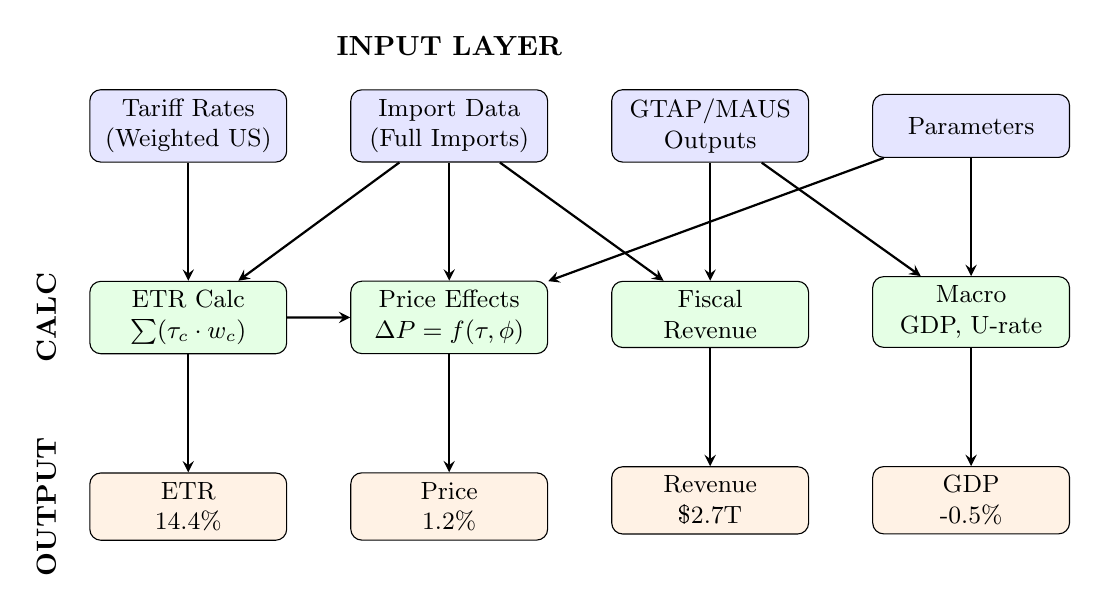
\begin{tikzpicture}[
    node distance=0.8cm,
    box/.style={rectangle, draw, rounded corners, minimum width=2.5cm, minimum height=0.8cm, align=center, font=\small},
    inputbox/.style={box, fill=blue!10},
    calcbox/.style={box, fill=green!10},
    outputbox/.style={box, fill=orange!10},
    arrow/.style={->, thick, >=stealth}
]

% Input layer
\node[inputbox] (tariffs) {Tariff Rates\\(Weighted US)};
\node[inputbox, right=of tariffs] (imports) {Import Data\\(Full Imports)};
\node[inputbox, right=of imports] (gtap) {GTAP/MAUS\\Outputs};
\node[inputbox, right=of gtap] (params) {Parameters};

% Calculation layer
\node[calcbox, below=1.5cm of tariffs] (etr) {ETR Calc\\$\sum(\tau_c \cdot w_c)$};
\node[calcbox, below=1.5cm of imports] (price) {Price Effects\\$\Delta P = f(\tau, \phi)$};
\node[calcbox, below=1.5cm of gtap] (fiscal) {Fiscal\\Revenue};
\node[calcbox, below=1.5cm of params] (macro) {Macro\\GDP, U-rate};

% Output layer
\node[outputbox, below=1.5cm of etr] (out1) {ETR\\14.4\%};
\node[outputbox, below=1.5cm of price] (out2) {Price\\1.2\%};
\node[outputbox, below=1.5cm of fiscal] (out3) {Revenue\\\$2.7T};
\node[outputbox, below=1.5cm of macro] (out4) {GDP\\-0.5\%};

% Arrows
\draw[arrow] (tariffs) -- (etr);
\draw[arrow] (imports) -- (etr);
\draw[arrow] (imports) -- (price);
\draw[arrow] (params) -- (price);
\draw[arrow] (etr) -- (price);
\draw[arrow] (gtap) -- (fiscal);
\draw[arrow] (imports) -- (fiscal);
\draw[arrow] (gtap) -- (macro);
\draw[arrow] (params) -- (macro);

\draw[arrow] (etr) -- (out1);
\draw[arrow] (price) -- (out2);
\draw[arrow] (fiscal) -- (out3);
\draw[arrow] (macro) -- (out4);

% Labels
\node[above=0.3cm of imports, font=\bfseries] {INPUT LAYER};
\node[left=0.3cm of etr, font=\bfseries, rotate=90, anchor=south] {CALC};
\node[left=0.3cm of out1, font=\bfseries, rotate=90, anchor=south] {OUTPUT};

\end{tikzpicture}
\end{center}

%==============================================================================
\section{External Model Dependencies}
%==============================================================================

The following data are pasted from external model runs and cannot be computed within the spreadsheet:

\begin{longtable}{llp{7cm}}
\toprule
\textbf{Model} & \textbf{Sheet} & \textbf{Variables} \\
\midrule
\endhead
GTAP & \texttt{F5 Foreign GDP!H} & GDP effects by region (\texttt{qgdp}) \\
GTAP & \texttt{F4 US Sector Output!X} & Output changes by sector \\
GTAP & \texttt{ricco\_price\_effects} cols AS--BB & Price/quantity effects \\
MAUS & \texttt{F3 GDP!T} & Quarterly GDP with tariffs \\
MAUS & \texttt{F3 GDP!W} & Quarterly unemployment with tariffs \\
MAUS & \texttt{F3 GDP!V} & Quarterly payrolls with tariffs \\
\bottomrule
\end{longtable}

%==============================================================================
\section{Key Formulas for R Conversion}
%==============================================================================

\subsection{Weighted Effective Tariff Rate}

\begin{lstlisting}[language=R]
weighted_etr <- sum(country_etr * import_weights) / sum(import_weights)
\end{lstlisting}

\subsection{Price Effect}

\begin{lstlisting}[language=R]
price_effect <- (etr * -usd_offset * goods_share * import_share) +
                (etr * import_share * goods_share * (1 + passthrough))
\end{lstlisting}

\subsection{Net Revenue}

\begin{lstlisting}[language=R]
gross_revenue <- new_duties - baseline_duties
net_revenue <- gross_revenue * (1 - compliance_effect - income_effect)
\end{lstlisting}

\subsection{GDP Impact (Q4-Q4)}

\begin{lstlisting}[language=R]
gdp_impact <- ((tariff_gdp_q4 / tariff_gdp_q4_prior) /
               (baseline_gdp_q4 / baseline_gdp_q4_prior) - 1) * 100
\end{lstlisting}

\subsection{Sector Effect}

\begin{lstlisting}[language=R]
sector_effect <- sum(output_weight * gtap_effect * sector_flag) /
                 sum(output_weight * sector_flag)
\end{lstlisting}

%==============================================================================
\section{Vestigial Elements}
%==============================================================================

The following elements can be ignored during R conversion:

\begin{itemize}
    \item \texttt{\_\_123Graph\_*} named ranges (Lotus 1-2-3 legacy)
    \item External links to old CBO/Yale SharePoint files
    \item Sheets marked with \texttt{IGNORE>>>}
    \item VBA macros in \texttt{vbaProject.bin} (primarily UI automation)
\end{itemize}

\vfill
\begin{center}
\textit{Generated from analysis of} \texttt{ricco\_tariffs\_11-17.xlsm}\\
January 5, 2026
\end{center}

\end{document}
